\section{Precision Test}
Once the application was developed, the datalogger was used to gather new data such that a precision test could be performed.
Data was recorded in distances of $1$, $2$, $25$, and $50$ meters.
These data were used to determine the correctness of the output given by the application.

Tables showing the test results can be seen in \appref{app:precision-tests}.
The majority of the tests showed that the application underestimated the calculated positions and the average calculated position was $46.1\%$ of the actual position.
The percent deviation ranged from $22.8\%$ to $164.1\%$, however, only $6$ calculated positions were above $70\%$ while $81$ were below $70\%$.
To summarize the percent deviation, a bar chart was made to show an overview of the data, see \figref{figure:acc-histo}.
%Hamuns ekstra edit End:

Various reasons for this underestimation could be the filters suppressing the accelerations, the rotation of the phone still having affect on the accelerations, or that the sensor readings in general measure too low values.

This underestimation could be corrected in various ways.
One way could be to scale the position with a factor, or to make further adjustments in the actual implementation.
Some of these adjustments are discussed in \chapref{chapter:discussion}.

\begin{figure}[H]
	\centering
	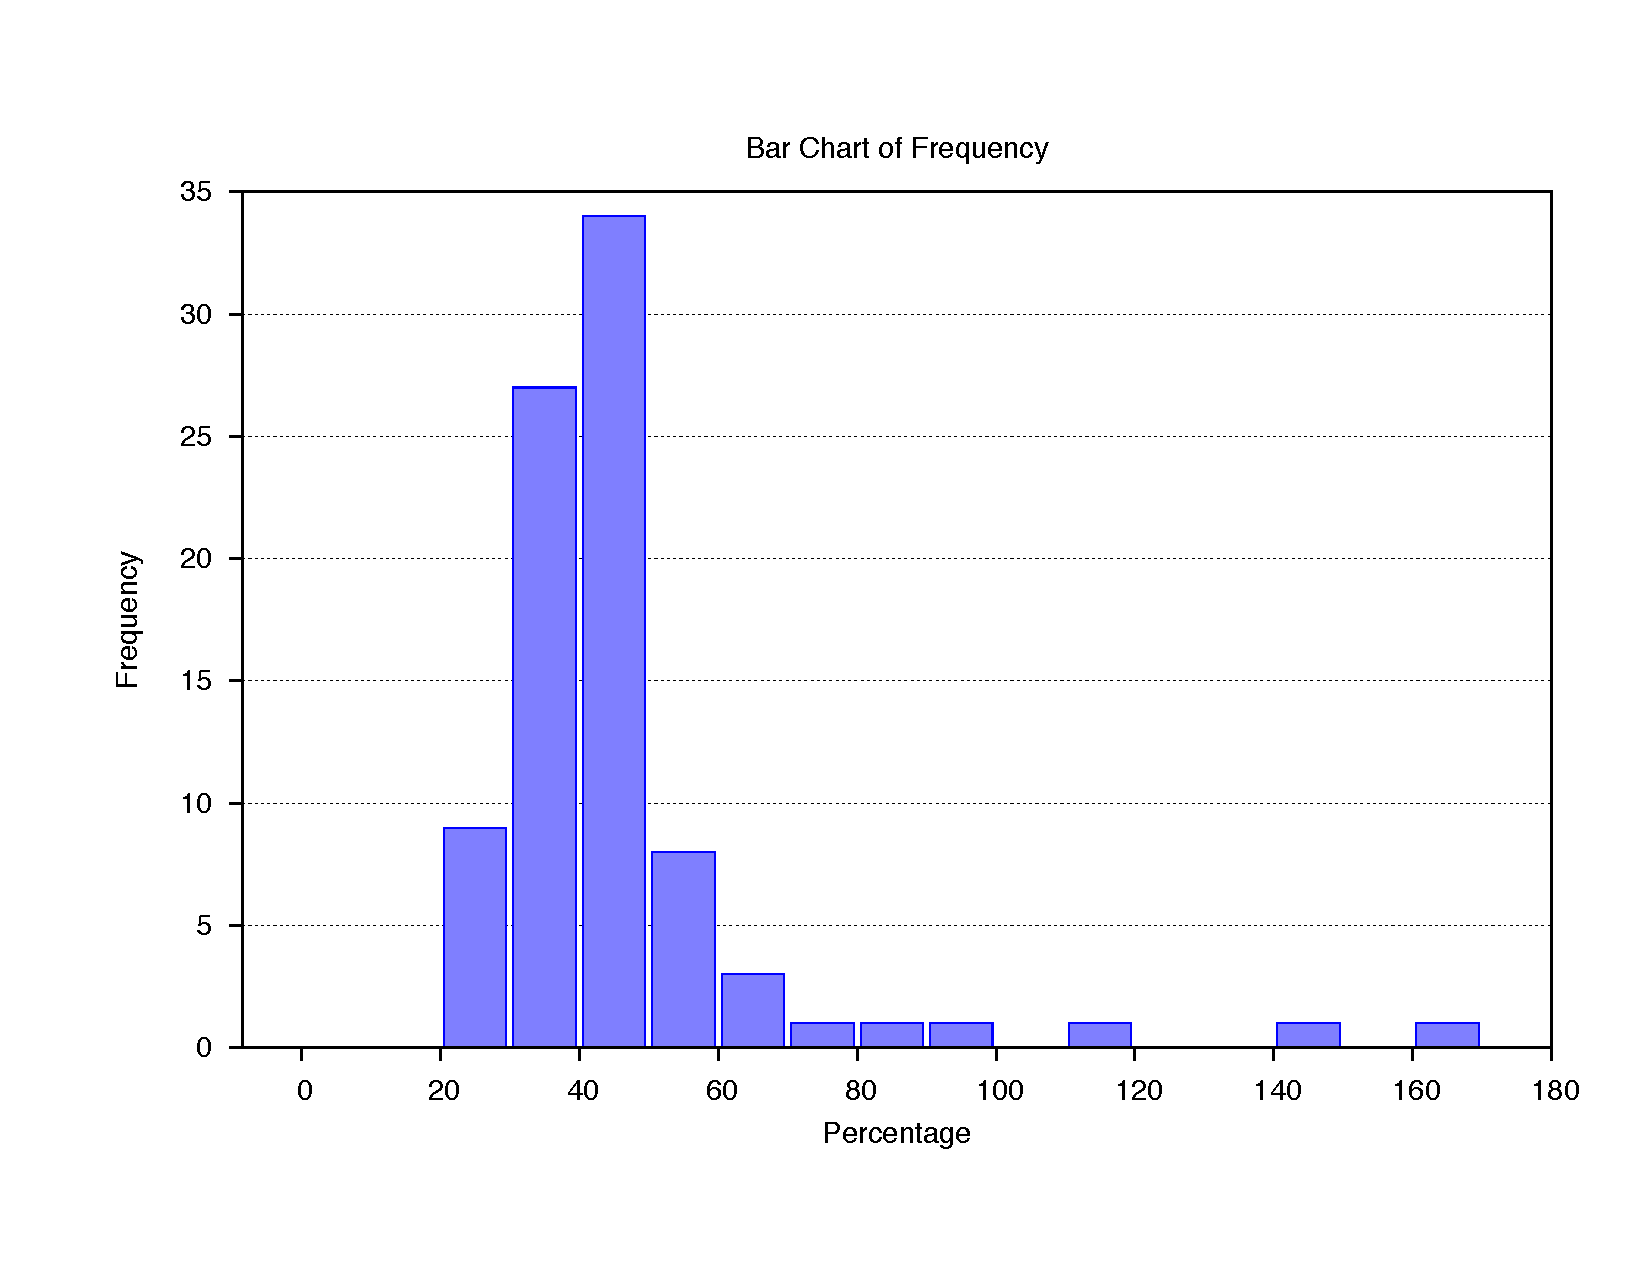
\includegraphics[scale=0.5, trim = 0cm 2cm 0cm 2cm, clip]{media/gnuplot/barchart.pdf}
	\caption{A bar chart for the percent deviation range and how many times it has been observed.}
	\label{figure:acc-histo}
\end{figure}